\section{Results}

\subsection{Does Randomization Make Pipelining More Robust?}
Compare to best single pipeline, worst single pipeline, and current state of the art.
We should find that a randomized execution is much better than the worst and hopefuly comparable to the best.
In some cases, it may be better than the best, but it should never be worse than the worst.

Dataset: MS Academic 
Operations: Filter and Deduplicate

Dataset: Yelp 
Operations: String Clean, City Format, Deduplicate

Dataset: Product 
Operations: identify sku if exists, string clean, Deduplicate

\begin{figure}[t]\vspace{-1.8em}
\centering
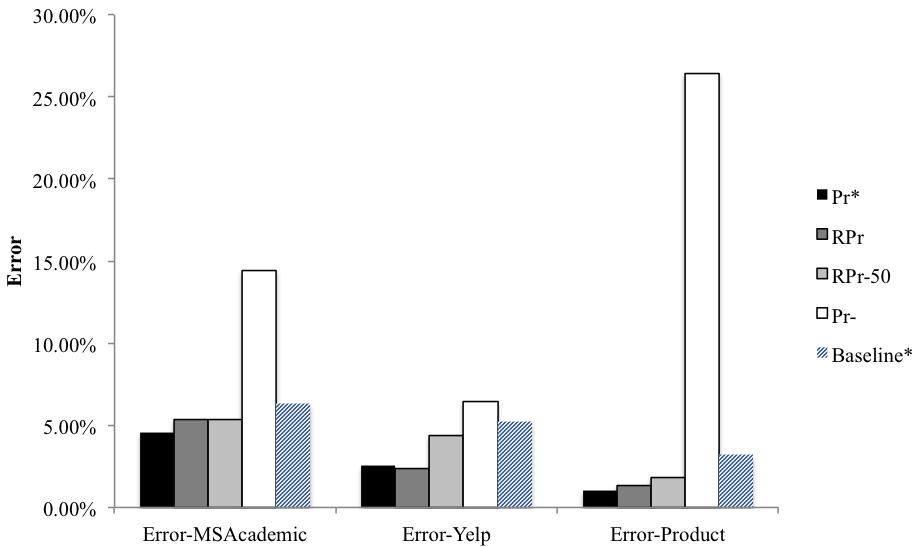
\includegraphics[scale=0.4]{fig1.png}
\caption{}
\label{exp:ms-academic-ranking}
\end{figure}

\subsection{How does this vary with random error in the operators?}
Should show that the more unreliable the data cleaning is the more that our approach benefits.

Introduce varying amount of random error (hashed so consistent between runs) into the ``city formatting" fix for the yelp dataset:

\begin{figure}[t]\vspace{-1.8em}
\centering
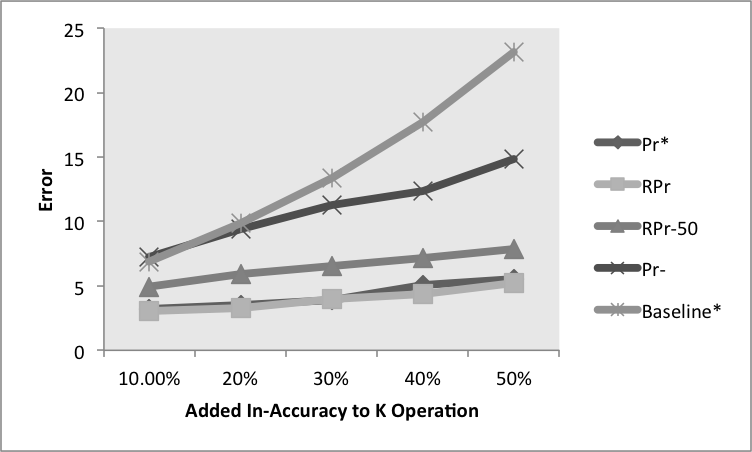
\includegraphics[scale=0.5]{fig2.png}
\caption{}
\label{exp:ms-academic-ranking}
\end{figure}

Introduce varying amound of random error (hashed so consistent between runs) into an extra dedup operation.

\begin{figure}[t]\vspace{-1.8em}
\centering
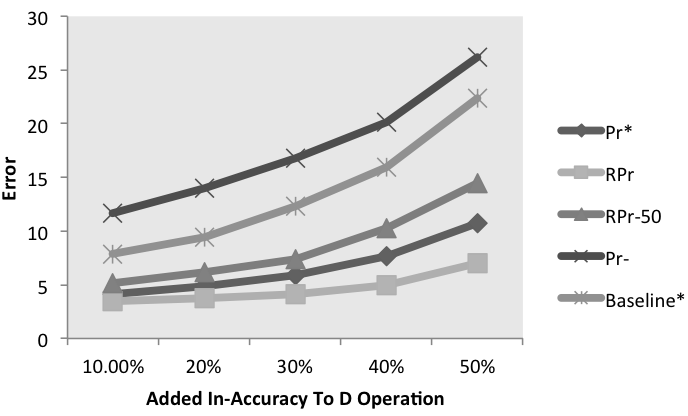
\includegraphics[scale=0.5]{fig3.png}
\caption{}
\label{exp:ms-academic-ranking}
\end{figure}

\subsection{Runtime-Accuracy Tradeoff}
Execute more samples and show how the accuracy improves.

\begin{figure}[t]\vspace{-1.8em}
\centering
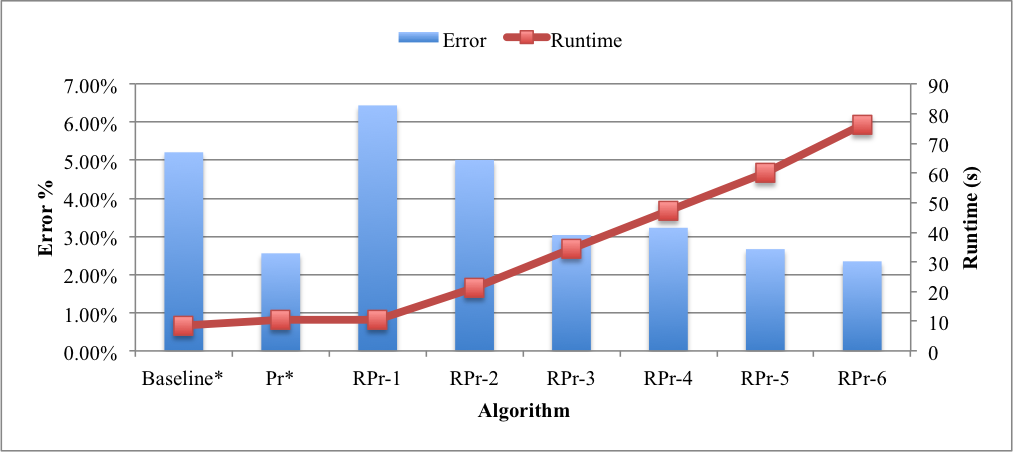
\includegraphics[scale=0.5]{fig4.png}
\caption{}
\label{exp:ms-academic-ranking}
\end{figure}


\subsection{Large-scale experiments}
Streaming correlation clustering. Show that at scale this technique can work and in a distributed environment.


